% !TEX encoding = UTF-8 Unicode

\documentclass[a4paper]{article}

\usepackage{color}
\usepackage{url}
\usepackage[T2A]{fontenc} % enable Cyrillic fonts
\usepackage[utf8]{inputenc} % make weird characters work
\usepackage{graphicx}

\usepackage[english,serbian]{babel}
%\usepackage[english,serbianc]{babel} %ukljuciti babel sa ovim opcijama, umesto gornjim, ukoliko se koristi cirilica

\usepackage[unicode]{hyperref}
\hypersetup{colorlinks,citecolor=green,filecolor=green,linkcolor=blue,urlcolor=blue}

%\newtheorem{primer}{Пример}[section] %ćirilični primer
\newtheorem{primer}{Primer}[section]

\begin{document}

\title{Bitcoin u 2022. godini\\ \small{Seminarski rad u okviru kursa\\Tehničko i naučno pisanje\\ Matematički fakultet}}

\author{Lazar\\ @alas.matf.bg.ac.rs\and Tanja\\@alas.matf.bg.ac.rs\and Aleksa Marković\\mi20244@alas.matf.bg.ac.rs\and Miljan Lješnjak\\mi22359@alas.matf.bg.ac.rs }
\date{21.~novembar 2022.}
\maketitle

\abstract{
U ovom tekstu je ukratko prikazana osnovna forma seminarskog rada. Obratite pažnju da je pored ove .pdf datoteke, u prilogu i odgovarajuća .tex datoteka, kao i .bib datoteka korišćena za generisanje literature. Na prvoj strani seminarskog rada su naslov, apstrakt i sadržaj, i to sve mora da stane na prvu stranu! Kako bi Vaš seminarski zadovoljio standarde i očekivanja, koristite uputstva i materijale sa predavanja na temu pisanja seminarskih radova. Ovo je samo šablon koji se odnosi na fizički izgled seminarskog rada (šablon koji \emph{morate} da ispoštujete!) kao i par tehničkih pomoćnih uputstava. 

\tableofcontents

\newpage

\section{Uvod}
\label{sec:uvod}
Kada budete predavali seminarski rad, imenujete datoteke tako da sadrže temu seminarskog rada, kao i prezimena članova grupe. Predaja seminarskih radova biće isključivo preko veb forme, a NE slanjem mejla. Link na formu će biti dat u okviru obaveštenja na strani kursa. Vodite računa da prilikom predavanja seminarskog rada predate samo one fajlove koji su neophodni za ponovno generisanje pdf datoteke. To znači da pomoćne fajlove, kao što su .log, .out, .blg, .toc, .aux i slično, \textbf{ne treba predavati}.

\section{Princip rada Bitcoin-a}
\label{sec:princip_rada}

Bitkoin \textbf{(eng. Bitcoin)} je izgradjen na distribuiranom digitalnom zapisu koji se zove Blokčejn \textbf{(eng. Blockchain)} (Slika \ref{fig:Blockchain}). Kao što naziv implicira, blokčejn predstavlja povezano telo podataka, sastavljeno od jedinica koje se nazivaju blokovi. Blokovi sadrže informacije o svakoj transakciji, uključujući datum i vreme, ukupnu vrednost, kupca i prodavca i jedinstveni identifikacioni kod za svaku razmenu. Unosi su nanizani hronološkim redom, stvarajući digitalan lanac blokova.
\\
\begin{figure}[h!]
\begin{center}

\includegraphics[scale=0.15]{Blockchain.jpg}
\end{center}
\caption{Blockchain}
\label{fig:Blockchain}
\end{figure}

\newpage
Jednom kada se blok doda u blokčejn, on postaje dostupan svima koji žele da ga vide, delujući kao javna knjiga transakcija kriptovaluta.
\\
Blokčejn je decentralizovan, što znači da ga ne kontroliše nijedna organizacija. Niko ga ne poseduje, ali svako može da ga koristi i da doprinese njegovom razvoju. Kako ga različiti ljudi ažuriraju, kopija koju pojedinac poseduje se takodje ažurira.
\\
\\
Iako ideja da svako može da uredjuje blokčejn može zvučati rizično, to je zapravo ono što Bitcoin čini pouzdanim i sigurnim.
\\
\\
\\
Da bi blok trasakcije bio dodat Bitcoin blok lancu, mora da bude verifikovan od strane velikog broja vlasnika Bitcoin-a, a za svakog korisnika koristi se jedinsveni verifikacioni kod.
\\
\\
Verifikacioni kodovi su dugi, nasumični brojevi, što njihovo lažiranje ili zloupotrebu predstavlja izuzetno teškim. Nivo statističke nasumičnosti blokčejn verificionih kodova, koji su potrebni za svaku transakciju, u velikoj meri smanjuje rizik da svako može da vrši razne zloupotrebe i lažne bitcoin transakcije.


\clearpage
\section{Socioekonomski uticaj Bitcoin-a}

\subsection{Energija}

Rudarenje bitcoin-a zahteva mašine sa puno procesorske snage, pa je samim tim velika potrošnja energije neophodna da bi se hardver poput grafičke kartice pokretao, iako su novije komponente sve više i više energetski efikasne. Pored mašina, rudari i kompanije za rudarenje sa velikim sistemima često imaju potrebu za jakim uređajima za rashlađivanje koje potpomažu performanse. Energija koja se troši prilikom rudarenja bitcoin-a raste zajedno sa bitcoin mrežom.

Gledajući energiju koja se godišnje potroši na rudarenje bitcoin-a, možemo videti da ona prevazilazi količine koje godišnje potroše čitave države. Bitcoin je 2019. godine potrošio oko 87.1 TWh\footnote{Teravat-sat} električne energije, što je više nego što je te godine potrošila Belgija.  \cite{energijapotrosnja}


Ovolika potrošnja energije ima mnogo posledica. Mapa rudarenja bitcoin-a u periodu 2019-2020, na osnovu geolokacije rudara ukazuje da je skoro 70\% rudarenja rađeno u Kini. \cite{energijakina}

Kako se Kina najviše oslanja na energiju dobijenu iz fosilnih goriva, može se reći da bitcoin dovodi do emitovanja značajne količine gasova staklene bašte.

Ova otkrića imala su negativan efekat na reputaciju bitcoin-a, pošto sve više ljudi brine o klimatskim promenama i preferira zelenu energiju. Jedan od izazova za bitcoin biće potrošnja energije i prelaženje na čistije i održivije energije.


\subsection{Cene i zalihe hardverda }

Grafičke kartice jedna su od najčešćih hardverskih komponenti koje se koriste za rudarenje bitcoin-a. Većina rudara koristi više od jedne grafičke kartice za njihov sistem, a česta je i pojava čitavih farmi (industrijski objekti namenjeni rudarenju). To je neophodno da bi rudarenje uopšte bilo isplativo i iz istog razloga rudari teže da nabave najnovije kartice po njihovom izlasku.

Ovo je jedan od razloga zbog kojih postoji nestašica grafičkih kartica, i to je problem koji se znatno pogoršava sa porastom popularnosti bitcoin-a i generalno kriptovaluta. Najnovije i najjače grafičke kartice većinski kupuju kompanije specijalizovane za rudarenje i individualni rudari. Maloprodaje iskorišćavaju činjenicu da proizvođači ne mogu da ispune ogromnu potražnju, te podižu cene do čak tri puta više od preporučene.

Bočni efekat ovog problema je veliki uticaj na polovno tržište grafičkih kartica. Kako nema grafičkih kartica u zalihama, rudari se okreću ovom tržištu i masovno kupuju polovne kartice, s obzirom da je često potrebno više starijih modela grafičkih kartica da bi bile isplative koliko i najnoviji modeli. Ovo iskorišćavaju i ljudi koji prodaju svoje korišćene kartice da podignu cene do te mere, da ih prodaju za više para nego što su ih platili nove.

Sve ovo skoro onemogućava prosečnom potrošaču da kupi grafičku karticu. U pokušaju da oslabe ove efekte, proizvođači uvode razne mere. NVIDIA, jedna od najvećih proizvođača grafičkih kartica, odlučila je da krene sa proizvodnjom grafičkih kartica specijalizovanih za rudarenje. Takođe je umanjila performanse rudarenja novih grafičkih kartica, koje su prvenstveno namenjene za video igrice, tako što im je umanjila hash rate. Ovo je dovelo do kritika od strane potrošača, na račun toga da NVIDIA svoju pažnju posvećuje grafičkim karticama namenjenim za rudarenje, dok stare linije ostavlja po strani. Takođe su ove odluke kritikovane da nove grafičke kartice neće imati preprodajnu vrednost i da će biti jednokratne.

\subsection{Monetarni sistem i politika}

Trenutno bitcoin skoro da nema uticaj na monetarne sisteme, s obzirom da je tržišna kapitalizacija bitcoin-a u svom vrhuncu bila oko 1.2 biliona američkih dolara, što je više od 5 puta manje od tržišne kapitalizacije bankarskog tržišta. Takođe, čak i centralne banke koje eksperimentišu sa kriptovalutama ne planiraju da koriste blokchain za njihove projekte, jer ga smatraju nestabilnim za infrastrukturu nacionalnih valuta. Kako se bitcoin oslanja na blokchain to ga čini nepogodnim, i samim tim neće imati uticaj na buduće planove monetarnog sistema.

Neke vlade se osećaju ugroženo od strane bitcoin-a iz razloga što bitcoin nema centralnu vlast i zato što može da destabilizuje autoritet centralnih banaka ili čak i samih vlada. Anonimnost koju pruža bitcoin može se koristiti za zaobilaženje raznih kontrola, pranje novca ili ilegalnu kupovinu. Zbog toga političari neretko ukazuju na probleme i mane bitcoin-a, poput potrošnje energije, sa ciljem da pokvari poverenje ljudi u njega. Sa druge strane, neki političari biraju da kritikuju način na koji se bitcoin oporezuje i razmenjuje sa ciljem da odvrate ljude od investiranja. To ne ide u prilog bitcoin-u, koji još uvek većina investitora smatra za rizičnu investiciju.


\clearpage

\section{Osnovna uputstva}
Vaš seminarski rad mora da sadrži najmanje jednu sliku, najmanje jednu tabelu i najmanje tri reference u spisku literature. \textbf{Dužina seminarskog rada treba da bude:}
\begin{itemize}
\item Ukoliko tim ima dva člana, tada od 3 do 5 strana
\item Ukoliko tim ima tri člana, tada od 4 do 6 strana
\end{itemize} 

Ко жели, може да пише рад ћирилицом. У том случају, неопходно је да су инсталирани одговарајући пакети: texlive-fonts-extra, texlive-latex-extra, texlive-lang-cyrillic, texlive-lang-other. 

Nemojte koristiti stari način pisanja slova, tj ovo:
\begin{verbatim}
\v{s} i \v{c} i \'c ...
\end{verbatim}
Koristite direknto naša slova:	
\begin{verbatim}
š i č i ć ... 
\end{verbatim}


\section{Engleski termini i citiranje}	
\label{sec:termini_i_citiranje}

Na svakom mestu u tekstu naglasiti odakle tačno potiču informacije. Uz sve novouvedene termine u zagradi naglasiti od koje engleske reči termin potiče. 

Naredni primeri ilustruju način uvođenja enlegskih termina kao i citiranje.

\begin{primer}
Problem zaustavljanja (eng.~{\em halting problem}) je neodlučiv \cite{haltingproblem}.
\end{primer}

\begin{primer}
Za prevođenje programa napisanih u programskom jeziku C može se koristiti GCC kompajler \cite{gcc}.
\end{primer}

\begin{primer}
 Da bi se ispitivala ispravost softvera, najpre je potrebno precizno definisati njegovo ponašanje \cite{laski2009software}. 
\end{primer}

Ukoliko za unos referenci koriste datoteku {\em seminarski.bib},  prevođenje u pdf format u Linux okruženju može se uraditi na sledeći način:
\begin{verbatim}
pdflatex TemaImePrezime.tex 
bibtex TemaImePrezime.aux 
pdflatex TemaImePrezime.tex 
pdflatex TemaImePrezime.tex 
\end{verbatim}
Prvo latexovanje je neophodno da bi se generisao {\em .aux} fajl. {\em bibtex} proizvodi odgovarajući {\em .bbl} fajl koji se koristi za generisanje literature. 
Potrebna su dva prolaza (dva puta pdflatex) da bi se reference ubacile u tekst (tj da ne bi ostali znakovi pitanja umesto referenci). Dodavanjem novih referenci potrebno je ponoviti ceo postupak.  


Broj naslova i podnaslova je proizvoljan. Neophodni su samo Uvod i Zaključak. Na poglavlja unutar teksta referisati se po potrebi. 
\begin{primer}
U odeljku \ref{sec:naslov1} precizirani su osnovni pojmovi, dok su zaključci dati u odeljku \ref{sec:zakljucak}.
\end{primer}




\section{Slike i tabele}
\label{slike_i_tabele}

Slike i tabele treba da budu u svom okruženju, sa odgovarajućim naslovima, obeležene labelom da koje omogućava referenciranje. 

\begin{primer} Ovako se ubacuje slika. Obratiti pažnju da je dodato i 
\begin{verbatim}
\usepackage{graphicx}
\end{verbatim}

\begin{figure}[h!]
\begin{center}
%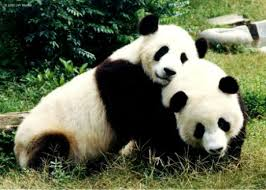
\includegraphics[scale=0.75]{pande.jpg}
\end{center}
\caption{Pande}
\label{fig:pande}
\end{figure}

Na svaku sliku neophodno je referisati se negde u tekstu. Na primer, na slici \ref{fig:pande} prikazane su pande. 
\end{primer}

\begin{primer} I tabele treba da budu u svom okruženju, i na njih je neophodno referisati se u tekstu. Na primer, u tabeli \ref{tab:tabela1} su prikazana različita poravnanja u tabelama.

\begin{table}[h!]
\begin{center}
\caption{Razlčita poravnanja u okviru iste tabele ne treba koristiti jer su nepregledna.}
\begin{tabular}{|c|l|r|} \hline
centralno poravnanje& levo poravnanje& desno poravnanje\\ \hline
a &b&c\\ \hline
d &e&f\\ \hline
\end{tabular}
\label{tab:tabela1}
\end{center}
\end{table}

\end{primer}





\section{Prvi naslov}
\label{sec:naslov1}


Ovde pišem tekst. 
Ovde pišem tekst. 
Ovde pišem tekst. 
Ovde pišem tekst. 
Ovde pišem tekst. 
Ovde pišem tekst. 
Ovde pišem tekst. 
Ovde pišem tekst. 


\subsection{Prvi podnaslov}
\label{subsec:podnaslov1}

Ovde pišem tekst. 
Ovde pišem tekst. 
Ovde pišem tekst. 
Ovde pišem tekst. 
Ovde pišem tekst. 
Ovde pišem tekst. 
Ovde pišem tekst. 

\subsection{Drugi podnaslov}
\label{subsec:podnaslov2}

Ovde pišem tekst. 
Ovde pišem tekst. 
Ovde pišem tekst. 
Ovde pišem tekst. 
Ovde pišem tekst. 
Ovde pišem tekst. 

\section{Drugi naslov}
\label{sec:naslov2}

Ovde pišem tekst. 
Ovde pišem tekst. 
Ovde pišem tekst. 
Ovde pišem tekst. 

\subsection{... podnaslov}
\label{subsec:podnaslovN}

Ovde pišem tekst. 
Ovde pišem tekst. 
Ovde pišem tekst. 
Ovde pišem tekst. 
Ovde pišem tekst. 
Ovde pišem tekst. 

\section{n-ti naslov}
\label{sec:naslovN}

Ovde pišem tekst. 
Ovde pišem tekst. 
Ovde pišem tekst. 
Ovde pišem tekst. 
Ovde pišem tekst. 

\subsection{... podnaslov}
\label{subsec:podnaslovK}

Ovde pišem tekst. 
Ovde pišem tekst. 
Ovde pišem tekst. 
Ovde pišem tekst. 
Ovde pišem tekst. 

\subsection{... podnaslov}
\label{subsec:podnaslovM}

Ovde pišem tekst. 
Ovde pišem tekst. 
Ovde pišem tekst. 
Ovde pišem tekst. 
Ovde pišem tekst. 

\section{Poslednji naslov}
\label{sec:naslovM}

Ovde pišem tekst. 
Ovde pišem tekst. 
Ovde pišem tekst. 
Ovde pišem tekst. 
Ovde pišem tekst. 
Ovde pišem tekst. 
Ovde pišem tekst. 
Ovde pišem tekst. 
Ovde pišem tekst. 

\section{Zaključak}
\label{sec:zakljucak}

Ovde pišem zaključak. 
Ovde pišem zaključak. 
Ovde pišem zaključak. 
Ovde pišem zaključak. 
Ovde pišem zaključak. 
Ovde pišem zaključak. 
Ovde pišem zaključak. 
Ovde pišem zaključak. 
Ovde pišem zaključak. 
Ovde pišem zaključak. 
Ovde pišem zaključak. 
Ovde pišem zaključak. 


\addcontentsline{toc}{section}{Literatura}
\appendix

\iffalse
\bibliography{seminarski} 
\bibliographystyle{plain}
\fi

\begin{thebibliography}{9}

\bibitem{energijapotrosnja} Alex de Vries. \emph{Bitcoin’s energy consumption is underestimated: A market dynamics approach}. Energy Res. Social Sci., vol. 70, Dec. 2020.

\bibitem{energijakina} Alex de Vries. \emph{IEA (2019), Bitcoin energy use - mined the gap}.  IEA, Paris, https://www.iea.org/commentaries/bitcoin-energy-use-mined-the-gap 

\bibitem{laski2009software} J. Laski and W. Stanley. \emph{Software Verification and Analysis}. Springer- Verlag, London, 2009.

\bibitem{gcc} Free Software Foundation. GNU gcc, 2013. on-line at: http://gcc. gnu.org/.

\bibitem{haltingproblem} A. M. Turing. \emph{On Computable Numbers, with an application to the Entscheidungsproblem}. Proceedings of the London Mathematical Society, 2(42):230–265, 1936.


\end{thebibliography}


\appendix
\section{Dodatak}
Ovde pišem dodatne stvari, ukoliko za time ima potrebe.
Ovde pišem dodatne stvari, ukoliko za time ima potrebe.
Ovde pišem dodatne stvari, ukoliko za time ima potrebe.
Ovde pišem dodatne stvari, ukoliko za time ima potrebe.
Ovde pišem dodatne stvari, ukoliko za time ima potrebe.


\end{document}
